\section{问题一：确定性储能经济调度}
\subsection{目标与求解}
已知负载与光伏预测时，确定144个时段的购电与充放电量，以
\begin{equation}\min J=\sum_tp_tG_t+\varepsilon\sum_t(C_t+D_t)\end{equation}
为目标，除共同储能约束外，满足逐段平衡
\begin{equation}G_t+V_t+D_t=L_t+C_t+W_t.\label{eq:q1balance}\end{equation}
$W_t$不获得售电收入。全部变量为连续变量，模型为线性规划，采用SciPy调用HiGHS求解。最优性限定于给定初始状态、输入预测和上述约束下的模型；并不表示考虑预测误差后的实际最优。报告购电费用$F=\sum p_tG_t$，不包含辅助惩罚。

\subsection{指定时段结果与储能策略}
\begin{table}[H]\centering\caption{问题一：指定时段与全天购电结果}\small\begin{tabularx}{\textwidth}{|Y|Y|Y|Y|Y|Y|}\hline 时间段&购电量&时间段&购电量&时间段&购电量\\\hline
10:00-10:10 & 0.0000 & 12:00-12:10 & 486.4029 & 14:00-14:10 & 0.0000\\\hline
16:00-16:10 & 394.9315 & 18:00-18:10 & 636.9826 & 20:00-20:10 & 0.0000\\\hline
\multicolumn{2}{|c|}{全天购电量/kWh}&59482.6990&\multicolumn{2}{c|}{全天购电费/元}&35126.9486\\\hline\end{tabularx}\end{table}

\begin{table}[H]\centering\small
\caption{问题一：储能充放电量（kWh）}
\begin{tabular}{lrr}\toprule
时间段 & 充电量 & 放电量\\\midrule
0:00-4:00 & 4500.0000 & 0.0000\\
4:00-8:00 & 833.3333 & 6365.8412\\
8:00-12:00 & 4787.9643 & 1702.9970\\
12:00-16:00 & 5286.0352 & 91.1014\\
16:00-20:00 & 0.0000 & 5780.1319\\
20:00-24:00 & 5333.3333 & 2859.8681\\
\bottomrule\end{tabular}\end{table}
日初与日末均为6000 kWh。凌晨低价阶段储能集中补能，日间吸收光伏富余，在高价时段释放电能。0:00--4:00累计充电4500 kWh；部分日间指定时段购电为零，体现光伏与储能共同承担负载，而非负载消失。

\begin{figure}[H]\centering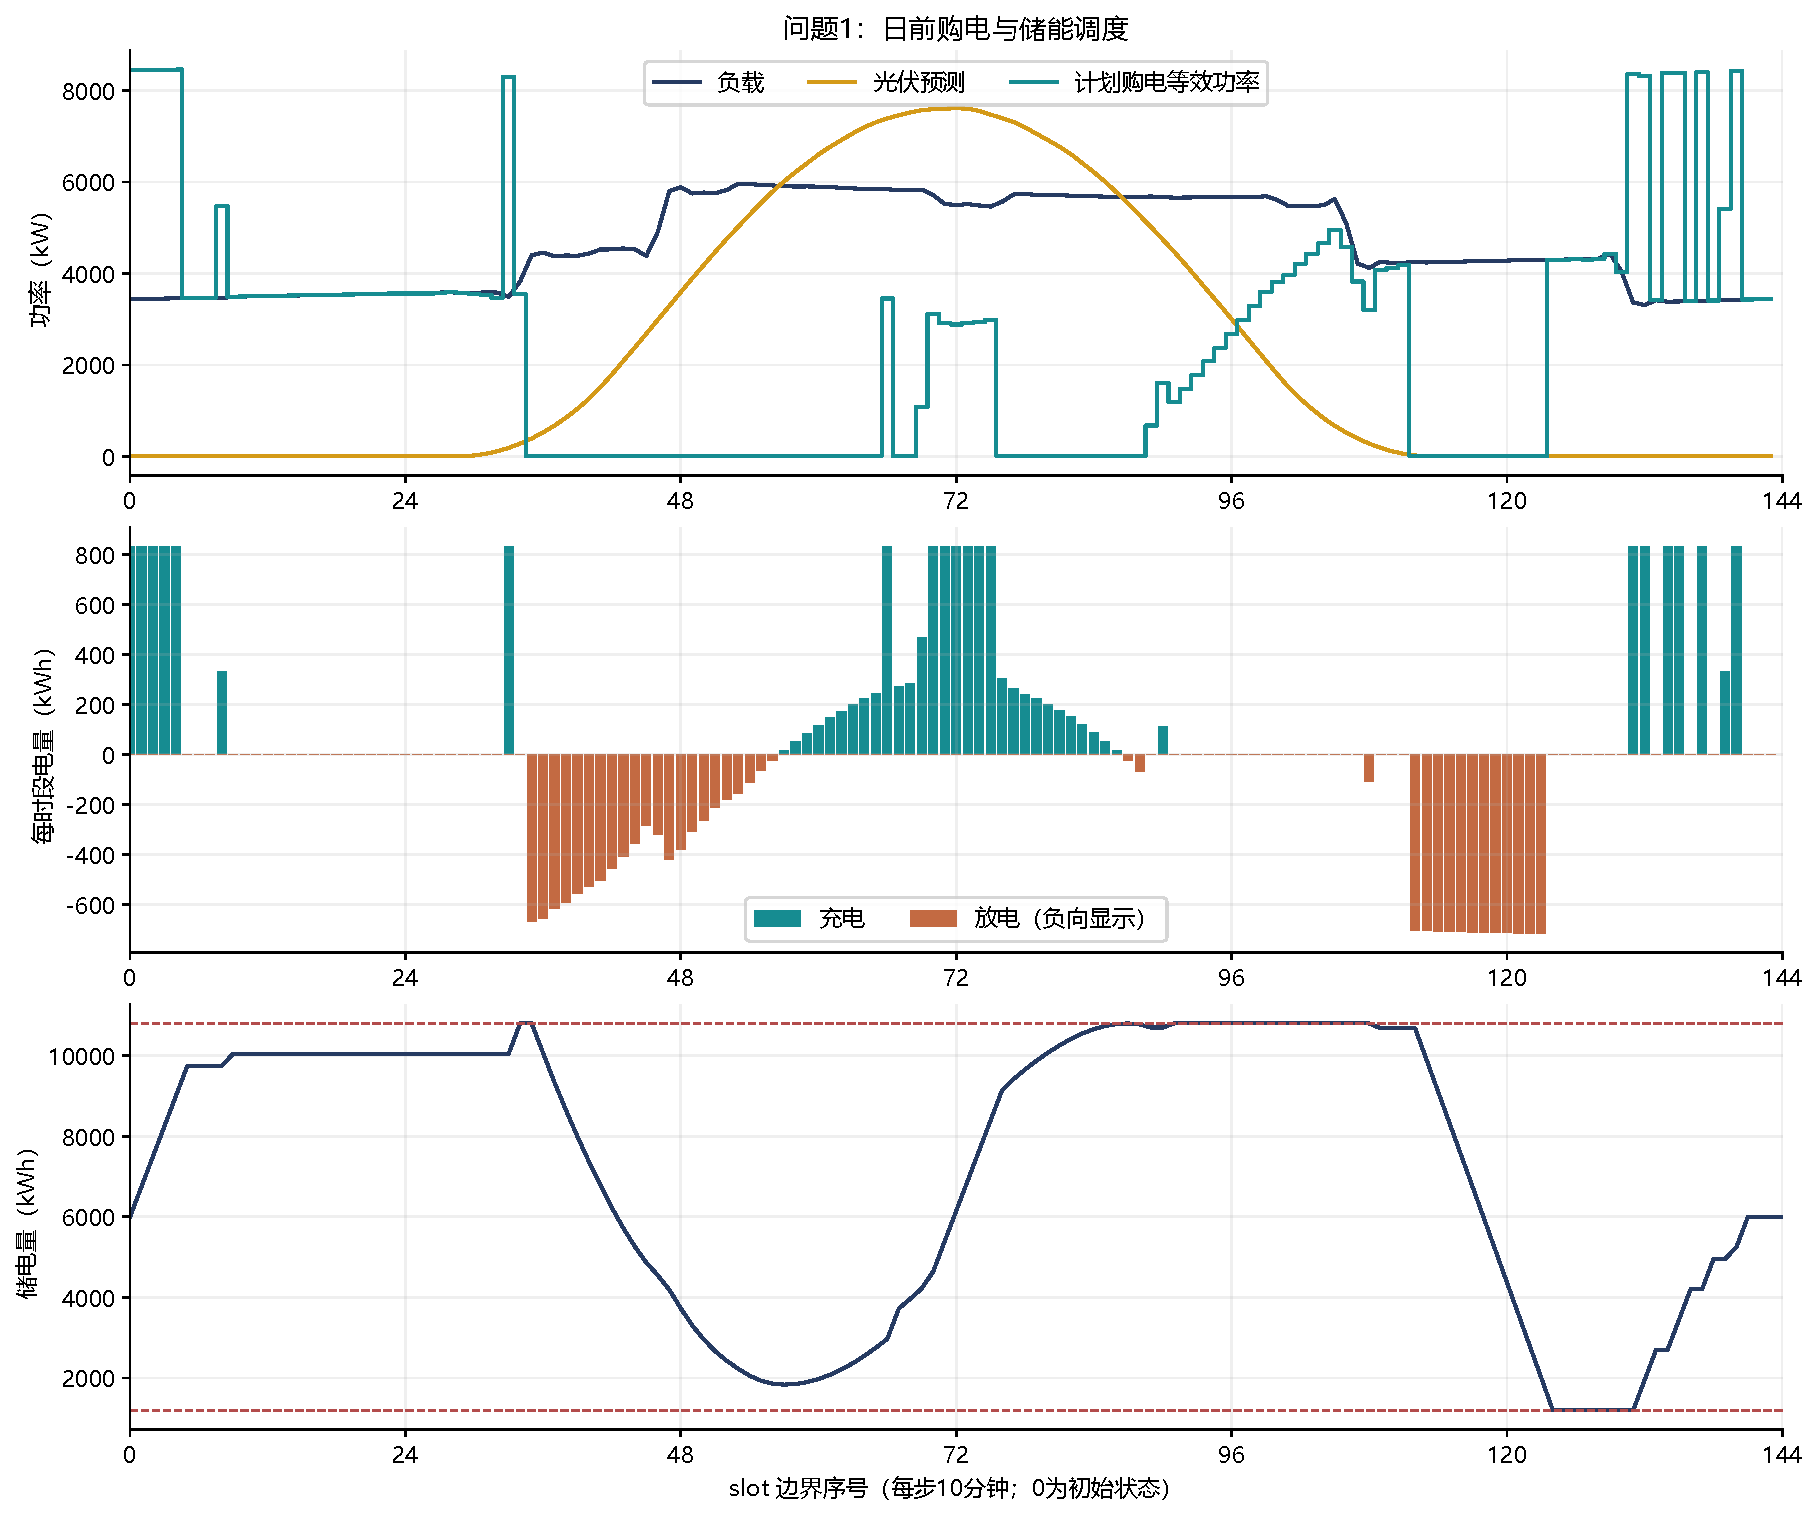
\includegraphics[width=.94\textwidth]{figures/q1_dispatch.pdf}
\caption{问题一的购电、光伏与储能调度；横轴按原始记录位置绘制}\end{figure}
\subsection{经济性与能量守恒}
无储能基准逐段购入正净负荷，购电量61789.9354 kWh，费用48052.0466元。储能优化使费用减少12925.0980元，降幅26.8981\%。该收益同时包含价格时移和光伏消纳改善，并非只来源于峰谷套利。
对状态转移求和，周期边界给出$\sum D_t=0.81\sum C_t$。逐段供需平衡求和后，外网购电等于净负荷加储能损耗及供能富余。当前重算解满足设备容量、功率、边界和能量平衡，且没有超过$10^{-6}$ kWh阈值的同时充放电。该检验支持本算例的物理可行性，不能代替任意参数下的互斥约束证明。
\FloatBarrier
